		%=================================================================
% IEEE "RECIPE-STYLE" TEMPLATE -- LabDST
%=================================================================
% What this is:
%   This template uses the CLASS and SYNTAX of IEEEtran (the same
%   one IEEE itself uses), but organizes the content with the KEY
%   SECTION STRUCTURE that MDPI uses (Introduction, Materials and
%   Methods, Design and Implementation, Results, Discussion,
%   Conclusions), because that structure explicitly explains WHAT
%   each section must contain -- not just how the LaTeX code works.
%
% Language:
%   The paper must be written entirely in English. This was decided
%   so the work can reach an international audience and match the
%   language IEEE venues expect. Keep the whole document in a single
%   language -- do not mix English and Spanish anywhere in the file,
%   including these instructions, figure/table captions, and code
%   comments.
%
% How to use it:
%   1. Every section below already contains guidance text explaining
%      what should go in that part of the paper. Replace it with your
%      actual content as you write.
%   2. The example figure uses fig1.png (already included in this
%      same folder). Replace it with your own figure, or add more
%      figures using the same block as a model.
%   3. The bibliography is EXTERNAL: it is defined in bibliography.bib
%      (in this same folder), and sources are cited with \cite{key}.
%      Do not type references by hand inside the .tex file.
%   4. Compile with pdflatex + bibtex/biber + pdflatex + pdflatex
%      (or "latexmk -pdf") so citations and the bibliography are
%      generated correctly.
%   5. Delete Section 0 ("How to Use This Template") completely
%      before submitting the final version: it is instructional only
%      and must not appear in the finished paper.
%=================================================================

\documentclass[lettersize,journal]{IEEEtran}
%--------------------
% Most common class options (uncomment/change as needed):
%--------------------
% [journal]     -> journal article (default format of this template)
% [conference]  -> conference paper
% [10pt,journal,compsoc] -> Computer Society journal article
% [9pt,technote]         -> brief note / correspondence
% Full option reference: see "IEEE Paper Template/main.tex"
% (the official IEEEtran guide) in the sibling folder of this template.

\usepackage{amsmath,amsfonts}
\usepackage{array}
\usepackage[caption=false,font=footnotesize]{subfig}
\usepackage{textcomp}
%\usepackage{stfloats}
\usepackage{url}
\usepackage{graphicx}
\usepackage{cite}
\usepackage{xcolor}
\usepackage{algorithm}
\usepackage{algpseudocode}
%\usepackage{enumitem}
%\usepackage{placeins}
\graphicspath{{figures/}}
\hyphenation{op-tical net-works semi-conduc-tor IEEE-Xplore}
\def\BibTeX{{\rm B\kern-.05em{\sc i\kern-.025em b}\kern-.08em
    T\kern-.1667em\lower.7ex\hbox{E}\kern-.125emX}}
\usepackage{balance}

\begin{document}

%=================================================================
\title{SOFIA: Modular Robotic Kinetic Surface for Human-Robot Interaction and Thermal-Constrained Actuator Characterization}

\author{Bernardo Orozco, Student 2, Student 3, Student 4, Student 5, Jorge A. Lizarraga, Graciela Baca, Luis Enrique Gonz{\'a}lez-Jim{\'e}nez and Luis F. Luque-Vega
\thanks{The authors are with the Department of Technological and
Industrial Processes, ITESO, Tlaquepaque 45604, Jalisco, Mexico.}}

\markboth{IEEE Transactions on Robotics / LabDST Academic Project}%
{Orozco \MakeLowercase{\textit{et al.}}: SOFIA: Modular Robotic Kinetic Surface for Human-Robot Interaction}

\maketitle

%=================================================================
\begin{abstract}
Modular robotic systems leverage repeatable electromechanical units to enable flexible, scalable, and reconfigurable architectures. In interactive human-robot installations, spatial tracking of human body posture and gestures provides intuitive stimulus-response dynamics. This paper presents SOFIA, an interactive modular robotic surface comprising sixteen electromechanical units, each providing two rotational degrees of freedom actuated by commercial MG90S servomotors. While commercial servomotors encapsulate internal closed-loop position control via pulse-width modulation (PWM), persistent angular errors caused by mechanical stalls, external disturbances, or fabrication tolerances induce thermal degradation and excessive power consumption. To investigate actuator reliability under persistent position error conditions, this work formulates an experimental characterization protocol assessing the thermal response of an MG90S under mechanical stall. Using an LM35 precision temperature sensor and a commanded reference angle, an empirical first-order thermal model is derived via logarithmic transformation and linear regression, yielding an estimated thermal time constant of $\tau \approx 80.6\text{ s}$ and a peak temperature exceeding $70^\circ\text{C}$. The proposed framework couples 3D real-time visual tracking with closed-loop kinematic control, providing direct evidence on the operational limits and thermal constraints required for reliable long-term deployment in modular robotic surfaces.
\end{abstract}

\begin{IEEEkeywords}
Modular robotics, Human-Robot Interaction (HRI), servomotor characterization, thermal modeling, bang-bang control, computer vision, kinematics.
\end{IEEEkeywords}

%=================================================================
\section{Introduction}
\label{sec:introduction}

\IEEEPARstart{M}{odular} robotics enables the design and construction of complex robotic systems from repeatable functional units that integrate mechanical, electronic, and control capabilities. This approach significantly streamlines manufacturing, system reconfiguration, and maintenance, while supporting distributed architectures where autonomous modules exchange information and share operational resources~\cite{seo2019modular}. Compared to monolithic, rigid robotic platforms, modular reconfigurable robots offer superior adaptability and permit functional units to be deployed across diverse spatial and kinematic configurations~\cite{seo2019modular}.

In parallel, socially interactive and human-robot interaction (HRI) systems incorporate perception and actuation mechanisms to establish continuous, non-verbal dialogue with human participants. Within this domain, posture, gestures, and body kinematics constitute vital communication channels for interpreting user intent and synthesizing reactive robotic behavior~\cite{fong2003social}. Consequently, modern kinetic robotic installations operate not merely as automated spatial mechanisms, but as interactive expressive surfaces capable of responding synchronously to multimodal human stimuli.

Within this framework, this paper introduces SOFIA, a modular robotic installation comprising sixteen electromechanical units arranged in a kinetic honeycomb array. Each module provides two rotational degrees of freedom (2-DOF) driven by dual metal-gear MG90S servomotors. Each unit incorporates dedicated onboard electronics for signal reception, trajectory interpolation, and actuator pulse generation. Global supervisory communication is established via Bluetooth Low Energy (BLE) and Wi-Fi, whereas inter-module synchronization is supported through an industrial RS-485 / Modbus bus.

The system relies on an ESP32-C3 microcontroller as the core processing and telemetry engine~\cite{espressif2024esp32c3}, coupled with PCA9685 16-channel 12-bit I$^2$C PWM controllers~\cite{nxp2024pca9685} to synthesize precise control pulses for the servomotors. Although commercial off-the-shelf (COTS) servomotors simplify spatial positioning, their internal closed-loop controllers remain completely encapsulated within the actuator housing. Consequently, while the supervisory system commands an angular setpoint via external 50~Hz PWM duty cycles, the internal drive strategy utilized to eliminate error between reference and actual shaft position is inaccessible to the designer.

This characteristic becomes critical when a servomotor experiences operational constraints where it cannot reach the commanded angular setpoint. In large-scale kinetic arrays composed of numerous densely packed modules, mechanical interference, fabrication tolerances, structural interference, or physical obstacles produce persistent, non-zero position errors. Under such conditions, internal driver behavior governs current draw, internal thermal dissipation, and long-term hardware reliability.

A classical control archetype relevant to bounded-input actuators under persistent saturation is bang-bang (on-off) control. Bang-bang strategies naturally arise in control problems subject to bounded actuation limits and represent a fundamental baseline for analyzing actuator dynamics under persistent error~\cite{boyd1991linear}. However, whether an embedded servomotor driver exhibits a quasi-bang-bang response cannot be established solely from external PWM waveforms.

To address this challenge, this paper experimentally characterizes the electromechanical and thermal behavior of the MG90S servomotor under persistent position error. By imposing a mechanical constraint on the output shaft and monitoring surface temperature with a precision LM35 sensor, this study extracts empirical first-order thermal models via linear regression. The primary working hypothesis posits that persistent angular error induces an observable thermal signature that quantitatively reflects actuator operational constraints. The core contribution of this work lies in combining a vision-driven modular robotic architecture for human-robot interaction with rigorous experimental actuator characterization, establishing thermal boundaries to guarantee operational reliability in kinetic surfaces.

\subsection{Related Work}
\label{sec:related_work}

Recent advances in interactive surfaces and vision-driven robotics have accelerated with lightweight machine learning inference frameworks. Qui{\~n}onez \textit{et al.}~\cite{quinonez2022mediapipe} demonstrated the efficacy of MediaPipe solutions for real-time 3D landmark estimation. Contemporary computer vision implementations leveraging MediaPipe~\cite{innovatiana2026mediapipe} and OpenCV~\cite{opencv2026library,omes2026deteccion} demonstrate how 21-point hand topologies and skeletal posture can be extracted in real time with minimal computational overhead. 

In modular and reconfigurable robotics, Seo \textit{et al.}~\cite{seo2019modular} established foundational taxonomy and scalability criteria for autonomous repeatable modules, emphasizing distributed coordination and power distribution challenges. Fong \textit{et al.}~\cite{fong2003social} surveyed social robotics, demonstrating that physical motion, non-verbal mirroring, and gestural responsiveness enhance user engagement. Nevertheless, existing kinetic installations frequently overlook actuator stall dynamics and internal thermal accumulation occurring across densely populated arrays. Boyd and Barratt~\cite{boyd1991linear} established theoretical boundaries for bounded controller actions; building upon these foundations, this research bridges the gap between high-level visual tracking and low-level physical actuator reliability.

\subsection{Formal Problem Formulation}
\label{sec:problem_formulation}

The SOFIA system requires coordinated spatial orientation of 32 independent servomotors across 16 electromechanical modules. Each actuator receives an angular reference setpoint $\theta_{\text{ref}}(t)$ and is commanded to achieve the target physical orientation $\theta(t)$.

The angular position error $e(t)$ for any given actuator is formally defined as:
\begin{equation}
e(t) = \theta_d(t) - \theta(t),
\label{eq:position_error}
\end{equation}
where $\theta_d(t) \in [\theta_{\min}, \theta_{\max}]$ corresponds to the desired (commanded) angular position, and $\theta(t)$ denotes the instantaneous actual angular position of the output shaft.

Under ideal, unconstrained operation, the internal feedback loop drives $e(t) \to 0$ within a settling time $t_s \in [75, 180]\text{ ms}$. However, when an external mechanical constraint prevents the actuator from reaching $\theta_d(t)$ such that $\theta(t) = \theta_{\text{stall}} \neq \theta_d(t)$, the error persists indefinitely:
\begin{equation}
e(t) = \theta_d(t) - \theta_{\text{stall}} = \Delta\theta_0 \neq 0, \quad \forall t \ge t_0.
\label{eq:persistent_error}
\end{equation}

When $e(t)$ persists, the internal H-bridge driver continuously supplies high current to the DC coreless motor in an attempt to minimize the tracking discrepancy. This condition causes significant Joule heating ($P_{\text{loss}} = I^2 R$) within the motor armature and driver silicon, inducing rapid thermal accumulation. Modeling this thermal profile and its associated time constant provides the quantitative foundation for actuator risk mitigation in the SOFIA array.

%=================================================================
\section{Materials and Methods}
\label{sec:methods}

Table~\ref{tab:bom_sofia} summarizes the bill of materials for the SOFIA 16-module system, including each component's technical description, manufacturer, and country of origin.

\begin{table*}[ht]
	\centering
	\caption{Bill of Materials Summary for the SOFIA 16-Module System}
	\label{tab:bom_sofia}
	\scriptsize
	\renewcommand{\arraystretch}{1.3}
	\begin{tabular}{p{3.5cm} c p{6.5cm} p{3.0cm} p{3.0cm}}
		\hline
		\textbf{Component} & \textbf{Qty.} & \textbf{Technical description} & \textbf{Manufacturer} & \textbf{Country / Location} \\
		\hline
		MG90S Servomotor & 32 & Metal gear micro servo, rated torque 1.8--2.2~kgf$\cdot$cm at 4.8--6.0~V, evaluated angle range $\theta \in [19.3^\circ, 70.2^\circ]$, 50~Hz PWM control & TowerPro & Shenzhen, China \\
		
		Module Enclosure & 16 & 3D-printed PLA enclosure, custom SOFIA003 honeycomb design for 2-DOF module & In-house (LabDST) & Mexico City, Mexico \\
		
		M3 Fasteners (Various) & 64 & Stainless steel socket head cap screw, M3 $\times$ 10~mm, for servo and frame mounting & Generic & Mexico City, Mexico \\
		
		PCA9685 Servo Driver & 2 & 16-Channel 12-bit PWM I$^2$C driver module for 32 servomotors & NXP Semiconductors / Adafruit & Eindhoven, Netherlands \\
		
		ESP32-C3 Master MCU & 1 & 32-bit RISC-V microcontroller, 2.4~GHz Wi-Fi / Bluetooth 5 LE for trajectory generation & Espressif Systems & Shanghai, China \\
		\hline
	\end{tabular}
\end{table*}


\begin{table}[ht]
	\centering
	\caption{ESP32-C3 technical specifications and compliance assessment.}
	\label{tab:esp32c3}
	\scriptsize
	\renewcommand{\arraystretch}{1.2}
	\begin{tabular}{|p{1.4cm}|p{1.8cm}|p{1.8cm}|p{1.8cm}|}
		\hline
		\textbf{Component} &
		\textbf{Parameter} &
		\textbf{Value} &
		\textbf{Source}\\
		\hline
		
		ESP32-C3
		(Espressif Systems, v2.4) &
		Supply Voltage (VDDA, VDD3P3, VDD3P3\_RTC) &
		3.0--3.6 V; 3.3 V typical &
		Datasheet v2.4, Section 5.2, Table 5-2, p. 54 \\
		\hline
		
		ESP32-C3 &
		Cumulative Supply Current (IVDD) &
		0.5 A min. &
		Datasheet v2.4, Section 5.2, Table 5-2, p. 54\\
		\hline
		
		ESP32-C3 &
		Peak Wi-Fi Transmission Current &
		276--335 mA, depending on the operating mode &
		Datasheet v2.4, Section 5.6.1, Table 5-7, p. 56\\
		\hline
		
		ESP32-C3 &
		VIH: High-Level Input Voltage &
		0.75 $\times$ VDD min. &
		Datasheet v2.4, Section 5.4, Table 5-4, p. 55\\
		\hline
		
		ESP32-C3 &
		VIL: Low-Level Input Voltage &
		$-0.3$ to 0.25 $\times$ VDD V &
		Datasheet v2.4, Section 5.4, Table 5-4, p. 55\\
		\hline
		
		ESP32-C3 &
		Strapping Pins / Boot Configuration Pins &
		GPIO2, GPIO8, and GPIO9. Their logic levels are sampled during reset to determine the boot mode. &
		Datasheet v2.4, Section 3, Boot Configuration, p. 30 \\
		\hline
		
		ESP32-C3 &
		GPIO8 and GPIO9 Boot-Time Levels &
		SPI Boot: GPIO9 = 1. Joint Download Boot: GPIO8 = 1 and GPIO9 = 0. The GPIO8 = 0, GPIO9 = 0 combination is not listed as a valid boot mode in Table 3-3. &
		Datasheet v2.4, Section 3.1, Table 3-3, p. 31\\
		\hline
		
		ESP32-C3 &
		Wi-Fi &
		2.4 GHz, IEEE 802.11 b/g/n &
		Datasheet v2.4, Features section, p. 3\\
		\hline
		
		ESP32-C3 &
		Bluetooth &
		Bluetooth 5 &
		Datasheet v2.4, Features section, p. 3 \\
		\hline
		
		ESP32-C3 &
		Operating Temperature &
		56 $^\circ$C &
		Datasheet v2.4, Section 1.2, Table 1-1, p. 12\\
		\hline
		
	\end{tabular}
\end{table}

\begin{table}[ht]
	\centering
	\caption{Servomotor MG90s technical specifications and compliance assessment.}
	\label{tab:MG90s}
	\scriptsize
	\renewcommand{\arraystretch}{1.2}
	\begin{tabular}{|p{1.2cm}|p{2.1cm}|p{1.8cm}|p{2.1cm}|}
		\hline
		\textbf{Component} &
		\textbf{Parameter} &
		\textbf{Value} &
		\textbf{Source}\\
		\hline
		
		MG90s &
		Supply and operating Voltage  &
		4.8 V – 6.0 V &
		MG90S datasheet, Tower Pro, p.2 \\
		\hline
		
		MG90s &
		Stall Torque &
		1.8 kgf·cm at 4.8V, 2.2 kgf·cm at 6V &
		MG90S datasheet, Tower Pro, p.1\\
		\hline
		
		MG90s &
		Operating Speed &
		0.1 s/60$^\circ$ at 4.8V, 0.08 s/60$^\circ$ at 6V &
		MG90S datasheet, Tower Pro, p.1\\
		\hline
		
		MG90s &
		Control Signal &
		PWM, orange wire; Vcc red; GND brown; 20 ms (50 Hz) period, 1--2 ms duty cycle &
		MG90S datasheet, Tower Pro, p.2\\
		\hline
		
		MG90s &
		Rotation Range &
		approximately 180 degrees (90$^\circ$ in each direction) &
		MG90S datasheet, Tower Pro, p.2\\
		\hline
		
		MG90s &
		Evaluated Angle Range (Experimental) &
		19.3$^\circ$ -- 70.2$^\circ$ (mean: 47.9$^\circ$) &
		LabDST test log (docs/experimental-data) \\
		\hline
		
		MG90s &
		Response Time (Experimental) &
		75 -- 180 ms &
		LabDST test log (docs/experimental-data) \\
		\hline
		
		MG90s &
		Dead Band Width &
		5 $\mu$s &
		MG90S datasheet, Tower Pro, p.2\\
		\hline
		
		MG90s &
		Operating Temperature &
		Not specified in datasheet &
		N/A\\
		\hline
		
		MG90s &
		Dimension \& Weight &
		22.5 $\times$ 12 $\times$ 35.5 mm approx.; 13.4 g &
		MG90S datasheet, Tower Pro, p.1\\
		\hline
		
	\end{tabular}
\end{table}

The servomotor operational limits and step response parameters were experimentally evaluated using the test protocol recorded in "docs/experimental-data/servomotor\_pruebas\_caracterizacion.xlsx". Under continuous PWM excitation at 50~Hz, the effective angular deflection spanned $\theta \in [19.3^\circ, 70.2^\circ]$ with a mean operating angle of $47.9^\circ$ and step response times ranging between $75\text{ ms}$ and $180\text{ ms}$.

\begin{table}[ht]
	\centering
	\caption{PCA9685 technical specifications and compliance assessment.}
	\label{tab:PCA9685}
	\scriptsize
	\renewcommand{\arraystretch}{1.2}
	\begin{tabular}{|p{1.4cm}|p{1.8cm}|p{1.8cm}|p{1.8cm}|}
		\hline
		\textbf{Component} &
		\textbf{Parameter} &
		\textbf{Value} &
		\textbf{Source}\\
		\hline
		
		PCA9685 (NXP Semiconductors, datasheet Rev. 4) &
		Supply Voltage ($V_{DD}$) &
		2.3--5.5 V &
		Datasheet Rev. 4, Section 2, Table 14, p. 38 \\
		\hline
		
		PCA9685 &
		PWM Resolution &
		12 bits (4096 steps) &
		Datasheet Rev. 4, Section 1, p. 1 \\
		\hline
		
		PCA9685 &
		Number of PWM Channels &
		16 independent channels &
		Datasheet Rev. 4, Section 1, p. 1 \\
		\hline
		
		PCA9685 &
		Communication Interface &
		I$^2$C Fast-mode Plus &
		Datasheet Rev. 4, Section 2, p. 2 \\
		\hline
		
		PCA9685 &
		Maximum I$^2$C Frequency &
		Up to 1 MHz &
		Datasheet Rev. 4, Section 2, p. 2 \\
		\hline
		
		PCA9685 &
		PWM Frequency Range &
		24 Hz -- 1526 Hz &
		Datasheet Rev. 4, Section 7.3.5, p. 25 \\
		\hline
		
		PCA9685 &
		Default PWM Frequency &
		Approximately 200 Hz &
		Datasheet Rev. 4, Table 8, p. 25 \\
		\hline
		
		PCA9685 &
		I$^2$C Address Configuration &
		A0--A5 pins, up to 62 devices &
		Datasheet Rev. 4, Section 7.1, p. 7 \\
		\hline
		
		PCA9685 &
		Output Current &
		25 mA per output &
		Datasheet Rev. 4, Table 13, p. 38 \\
		\hline
		
		PCA9685 &
		Total Output Current &
		400 mA maximum &
		Datasheet Rev. 4, Table 13, p. 38 \\
		\hline
		
		PCA9685 Module (UNIT Electronics) &
		Output Ports &
		16 PWM outputs with V+, GND and PWM signal &
		UNIT Electronics product specification \\
		\hline
		
		PCA9685 Module (UNIT Electronics) &
		Logic Voltage &
		3--5 V &
		UNIT Electronics product specification \\
		\hline
		
		PCA9685 Module (UNIT Electronics) &
		Servo Power Supply (V+) &
		External power supply for connected actuators &
		UNIT Electronics product specification \\
		\hline
		
		PCA9685 &
		Operating Temperature &
		$-40~^\circ\mathrm{C}$ to $+85~^\circ\mathrm{C}$ &
		Datasheet Rev. 4, Table 13, p. 38 \\
		\hline
		
	\end{tabular}
\end{table}

\subsection{Experimental Setup: Thermal Characterization under Persistent Error}
\label{sec:thermal_experiment}

To investigate the thermal behavior and reliability limits of the MG90S servomotors within the SOFIA architecture, an experimental testing apparatus was designed to record thermal dissipation under mechanical restriction. The test bench comprises:
\begin{enumerate}
\item An MG90S metal-gear servomotor powered by a regulated 5.0~V DC supply.
\item A 10~k$\Omega$ linear precision potentiometer utilized to set and modulate the commanded angular setpoint $\theta_{\text{ref}}(t)$.
\item A calibrated LM35 precision centigrade temperature sensor mechanically thermally coupled to the servomotor casing via thermal interface compound, providing an analog output of $10\text{ mV}/^\circ\text{C}$.
\item An acquisition node based on an ESP32 microcontroller acquiring angular commands and surface temperature $T_{\text{servo}}(t)$ at a sampling rate of $1\text{ Hz}$.
\end{enumerate}

A rigid mechanical boundary stop was rigidly fixed to the servomotor output horn to physically prevent the output shaft from reaching the commanded angular reference $\theta_{\text{ref}}(t)$, deliberately maintaining a persistent non-zero error condition: $e(t) = \theta_{\text{ref}}(t) - \theta_{\text{stall}} > 0$. Ambient room temperature $T_{\text{amb}}$ was monitored as the reference operating baseline.

The experimental characterization protocol was conducted in two sequential stages:
\begin{itemize}
\item \textbf{Trial 1 (Failure and Degradation Assessment):} The actuator was initialized at $T_{\text{amb}} = 21.37^\circ\text{C}$ and subjected to a persistent stall reference of $\theta_{\text{ref}} = 180^\circ$. The test proceeded continuously for $226\text{ s}$, until distinct audible abnormalities, gear strain, and subsequent actuator degradation occurred. The surface temperature climbed monotonically to a critical peak of $T_{\max} = 64.84^\circ\text{C}$.
\item \textbf{Trial 2 (Extended Thermal Accumulation and Cooling):} In an extended continuous run spanning $t \in [973.1, 1654.1]\text{ s}$ (682 data points), the actuator thermal profile was evaluated under varying commanded angular steps. Starting from $T_{\text{amb}} = 19.29^\circ\text{C}$, the casing reached a steady-state thermal maximum of $T_{\max} = 70.21^\circ\text{C}$ ($\Delta T = 50.92^\circ\text{C}$) before stabilization and subsequent cooling upon stall removal.
\end{itemize}

\subsection{First-Order Thermal Modeling and Parameter Identification}
\label{sec:thermal_modeling}

For the experimental characterization, the commanded angular position acts as the system input, $u(t) = \theta_d(t)$, while the recorded servomotor casing temperature represents the measured system output, $y(t) = T_s(t)$. Room ambient temperature is denoted as $T_a$.

In accordance with first-order thermal dynamics, the system is modeled in the Laplace domain by the empirical transfer function:
\begin{equation}
G_T(s) = \frac{T_s(s)}{\Theta_d(s)} = \frac{K_T}{\tau_T s + 1},
\label{eq:transfer_function}
\end{equation}
where $K_T$ represents the thermal steady-state gain ($^\circ\text{C}/\text{rad}$ or $^\circ\text{C}/^\circ$), and $\tau_T$ is the thermal time constant of the actuator.

In the time domain, the step response of this first-order system to a persistent commanded step input $\theta_d(t)$ is expressed as:
\begin{equation}
T_s(t) = T_a + (T_{ss} - T_a)\left(1 - e^{-t/\tau_T}\right),
\label{eq:first_order_time}
\end{equation}
where $T_{ss}$ represents the asymptotic steady-state temperature reached under continuous stall.

Following the identification methodology presented in the LabDST course lectures, the non-linear exponential response is transformed into a linear relationship:
\begin{equation}
\ln\left(T_{ss} - T_s(t)\right) = -\frac{1}{\tau_T} t + C,
\label{eq:linearized_thermal}
\end{equation}
where $C = \ln(T_{ss} - T_a)$ is a constant. Applying linear least-squares regression between $\ln(T_{ss} - T_s(t))$ and time $t$, the slope of the fitted line $m = -1/\tau_T$ provides the estimate of the thermal time constant:
\begin{equation}
\tau_T = -\frac{1}{m}.
\label{eq:identified_tau}
\end{equation}

Evaluating the empirical data from Trial 1 ($t \in [1, 226]\text{ s}$, $T_a = 21.37^\circ\text{C}$, $T_{ss} \approx 64.84^\circ\text{C}$) yields a regression slope of $m = -0.01241\text{ s}^{-1}$, corresponding to an identified thermal time constant of $\tau_T \approx 80.6\text{ s}$.

This quantitative identification confirms that when an MG90S servomotor enters an unmitigated mechanical stall, it reaches $63.2\%$ of its maximum thermal rise in approximately $80\text{ s}$, approaching destructive casing temperatures ($> 65^\circ\text{C}$) within 4 minutes. Because the internal driver continuously applies peak torque without internal thermal throttling, its behavior closely mirrors an unconstrained bang-bang controller under saturation.

\begin{figure}[!ht]
    \centering
    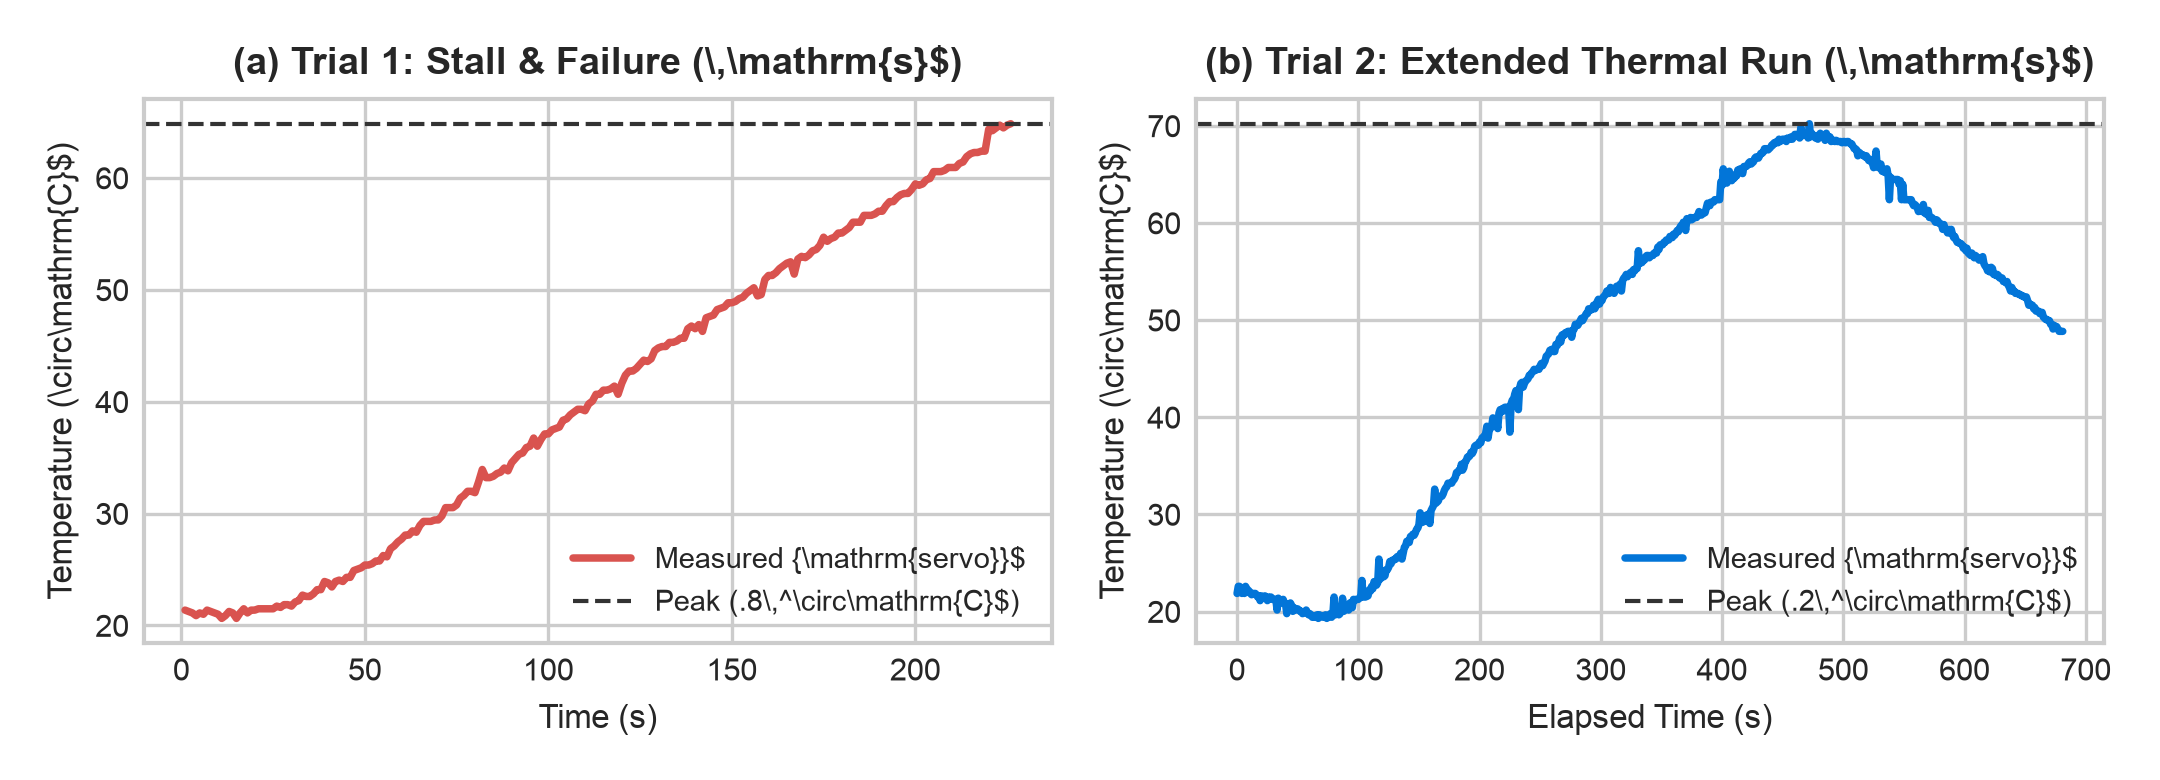
\includegraphics[width=\linewidth]{figures/fig_thermal_response}
    \caption{Experimental thermal characterization of the MG90S servomotor under persistent mechanical stall: (a) Trial 1 heating curve until audible failure at $t = 226\text{ s}$ ($T_{\max} = 64.84^\circ\text{C}$); (b) Trial 2 extended thermal cycle across 682 data points reaching peak steady-state temperature of $70.21^\circ\text{C}$.}
    \label{fig:thermal_response}
\end{figure}

%=================================================================
\section{Design and Implementation of the Technological Solution}
\label{sec:design}

The SOFIA technological solution integrates physical modular hardware, distributed electronics, and real-time vision-based kinematic coordination.

\subsection{System Architecture and Subsystems}
\label{sec:system_architecture}

The physical and functional architecture of the SOFIA platform is organized into three primary interconnected subsystems:
\begin{itemize}
\item \textbf{Perception and High-Level Control:} A host workstation executes an optimized real-time vision pipeline running on Python. It captures live camera feeds, performs 3D upper-body pose estimation and dual 21-point hand topology tracking, recognizes static and dynamic interaction gestures, and translates user coordinates $\mathbf{p}(t) \in \mathbb{R}^3$ into spatial target orientations.
\item \textbf{Master Communication and Telemetry:} An ESP32-C3 master microcontroller receives spatial setpoints via low-latency Wi-Fi / BLE communication and broadcasts synchronized module packets across an isolated RS-485 / Modbus serial bus.
\item \textbf{Distributed Modular Honeycomb Array:} 16 independent 2-DOF modules receive target angular pairs $(q_1, q_2)$. Actuation pulses are generated locally via PCA9685 12-bit PWM controllers, driving 32 MG90S metal-gear servomotors.
\end{itemize}

\subsection{Computer Vision Tracking and Dynamic Gesture Pipeline}
\label{sec:vision_pipeline}

The perception layer is developed using Python 3.11 with MediaPipe Tasks and OpenCV, structured into a modular, low-latency architecture:
\begin{enumerate}
\item \textbf{Real-Time 3D Landmark Extraction:} Using Google MediaPipe's Landmarker models in video mode, the system extracts 33 holistic body landmarks and two sets of 21 3D hand coordinates ($x, y, z$) with millisecond-accurate timestamps, achieving stable 30~FPS throughput on host CPUs.
\item \textbf{Rotation-Invariant Hand Topology:} Finger states are computed using 3D Euclidean distances between distal tips and the wrist base, normalized against palm scale $\lVert \mathbf{p}_{\text{wrist}} - \mathbf{p}_{\text{MCP}} \rVert$. This eliminates perspective distortion when fists face the camera.
\item \textbf{Dynamic Gesture Recognition Engine:} A modular coordination layer (\textit{GestureDetector}) arbitrates between static and dynamic interactions with strict temporal priority:
\begin{itemize}
\item \textit{Dynamic Wave (Saludo):} Tracks lateral palm oscillations (landmark 9 $X$-coordinate); requires at least 3 direction reversals and amplitude $> 0.05$ normalized units, prioritizing greeting over static open-hand detection.
\item \textit{Two-Handed RPS Game Intent (Intenci{\'o}n PPT):} Detects a horizontal flat palm as a reference plane and records 3 vertical fist-pump impacts using a finite-state machine ($d_{\text{contact}} < 0.17$ and $d_{\text{release}} > 0.20$ normalized units). A hysteresis hold filter prevents transient flickering with static rock or paper gestures.
\item \textit{Static Postures:} Detects two-handed heart geometries, scissors, open paper, and closed fists.
\end{itemize}
\end{enumerate}

\subsection{Electronic Interconnection and Current Hardware Stage}
\label{sec:hardware_stage}

In the current development stage (Corte 1, Discover $\to$ Learn), the physical electronic architecture is validated using commercial off-the-shelf (COTS) breakout boards on breadboards, directly interconnecting the ESP32-C3 microcontroller, dual PCA9685 PWM drivers, and external 5.0~V power rails. Custom printed circuit board (PCB) layout, routing, and fabrication remain open work for subsequent project phases (Make $\to$ Test), once the thermal boundaries and wiring constraints of the 16-module array are fully validated through the present prototype.

\subsection{Thermal Protection and Reliability Risk Mitigation}
\label{sec:risk_mitigation}

Based on the empirical thermal constant ($\tau \approx 80.6\text{ s}$) derived in Section~\ref{sec:thermal_modeling}, software-level watchdog limits are integrated into the SOFIA kinematic controller:
\begin{enumerate}
\item \textbf{Command Saturation Limiting:} Commanded angles are hard-bounded within the verified operational range $q_1, q_2 \in [19.3^\circ, 70.2^\circ]$ (mean: $47.9^\circ$) established in Table~\ref{tab:MG90s}.
\item \textbf{Stall Timeout Monitoring:} If an actuator target remains static under continuous high-load deflection for $\Delta t > 15\text{ s}$ ($< 0.2\,\tau$), the supervisory controller decrements the hold torque or enters an idle compliant mode, preventing cumulative temperature rise above the $55^\circ\text{C}$ safety ceiling.
\end{enumerate}

%=================================================================
\section{Results}
\label{sec:results}

\subsection{Kinematic Tracking Simulation}
\label{sec:results_simulation}

To validate the analytical kinematic model, a dynamic tracking
simulation of the 16-module SOFIA robotic honeycomb array was
conducted in a virtual 3D environment using the Unity engine~\cite{unity2023engine}. The objective was to evaluate
the coordinated orientation of the modules toward a moving target
coordinate $\mathbf{p}(t) \in \mathbb{R}^3$.

For each module $m_i$, the inverse kinematics procedure determines
the servo variables $(q_1,q_2)$ from the relative position of the
target with respect to the module base frame. The resulting joint
angles are constrained according to the permissible actuator range.
The complete inverse kinematics procedure is summarized in
Algorithm ~\ref{alg:sofia_ik}.

\begin{algorithm}[H]
\caption{SOFIA Module Inverse Kinematics}
\label{alg:sofia_ik}

\begin{algorithmic}[1]

\Require Module base origin $\mathbf{r}_{0,2}$, target coordinate
$\mathbf{p}$, joint angle limits
$[q_{1,\min},q_{1,\max}]$ and
$[q_{2,\min},q_{2,\max}]$

\Ensure Joint angles $q_1,q_2$

\State $\mathbf{r}_{2,p} \gets \mathbf{p} - \mathbf{r}_{0,2}$

\State $[u_x,u_y,u_z]^\top \gets
\mathbf{r}_{2,p}/\lVert\mathbf{r}_{2,p}\rVert$

\State $q_2 \gets \arcsin(u_x)$

\State $q_1 \gets \operatorname{atan2}(-u_y,u_z)$

\If{$q_1 < q_{1,\min}$}
    \State $q_1 \gets q_{1,\min}$
\ElsIf{$q_1 > q_{1,\max}$}
    \State $q_1 \gets q_{1,\max}$
\EndIf

\If{$q_2 < q_{2,\min}$}
    \State $q_2 \gets q_{2,\min}$
\ElsIf{$q_2 > q_{2,\max}$}
    \State $q_2 \gets q_{2,\max}$
\EndIf

\State \Return $q_1,q_2$

\end{algorithmic}
\end{algorithm}

Figure~\ref{fig:sofia_simulation} shows six representative frames
of the simulated tracking process. As the target moves through the
workspace, the modules progressively change their orientation,
maintaining the direction of their normal vectors
$\hat{r}_{2,3}^{(i)}$ toward the target position. The sequence
illustrates the coordinated response of the 16-module array during
different stages of the target trajectory.

\begin{figure}[!ht]
    \centering

    % Row 1
    \subfloat[]{
        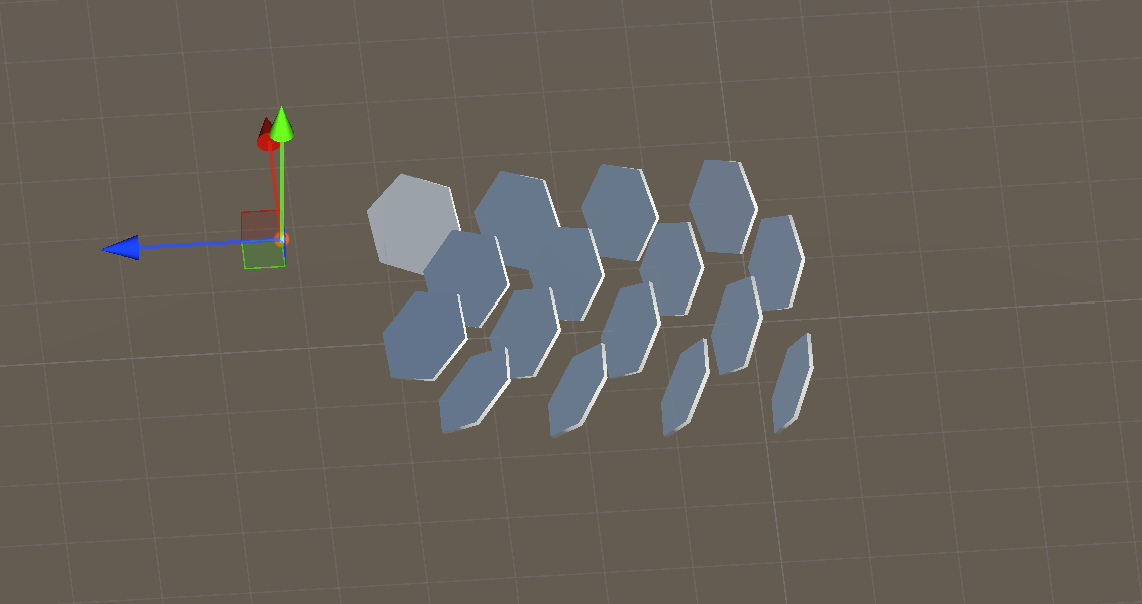
\includegraphics[
            width=0.47\linewidth
        ]{figures/fig_sim_1}
    }
    \hfill
    \subfloat[]{
        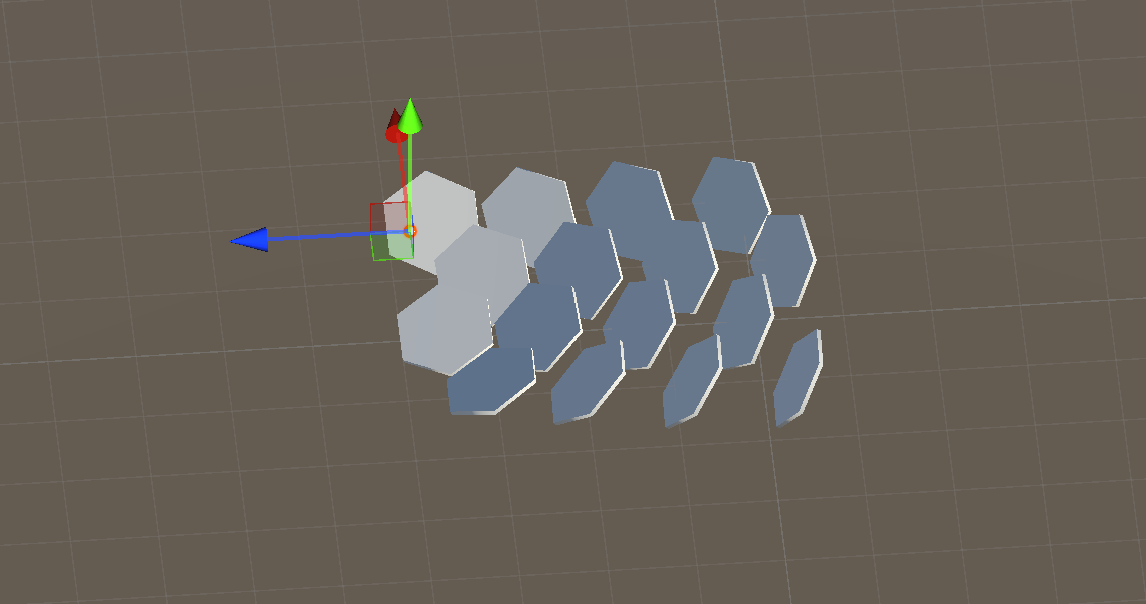
\includegraphics[
            width=0.47\linewidth
        ]{figures/fig_sim_2}
    }

    \par\vspace{2mm}

    % Row 2
    \subfloat[]{
        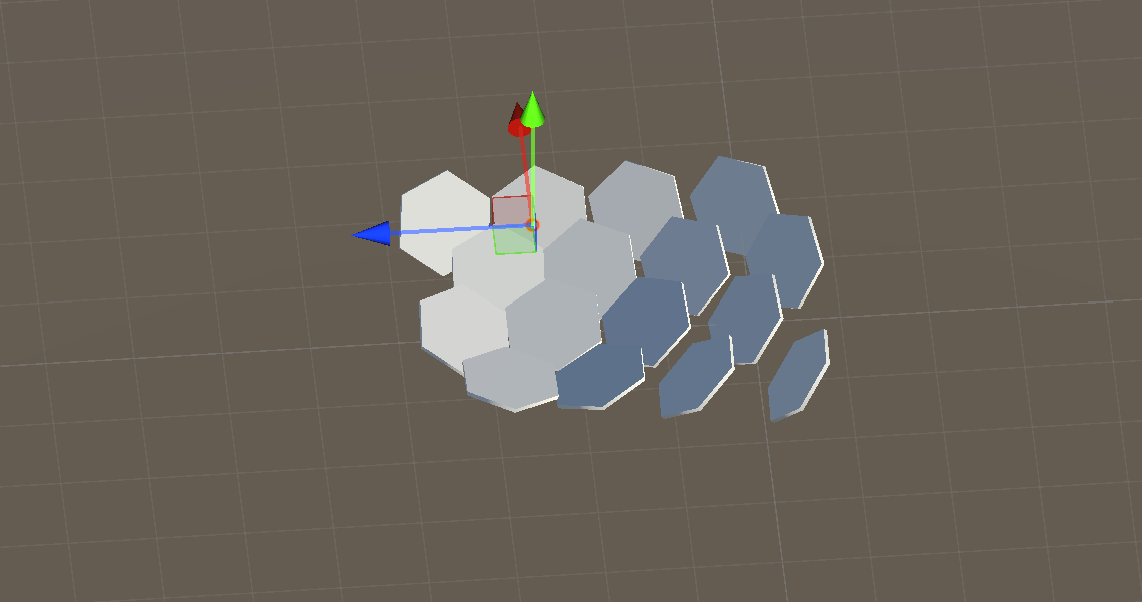
\includegraphics[
            width=0.47\linewidth
        ]{figures/fig_sim_3}
    }
    \hfill
    \subfloat[]{
        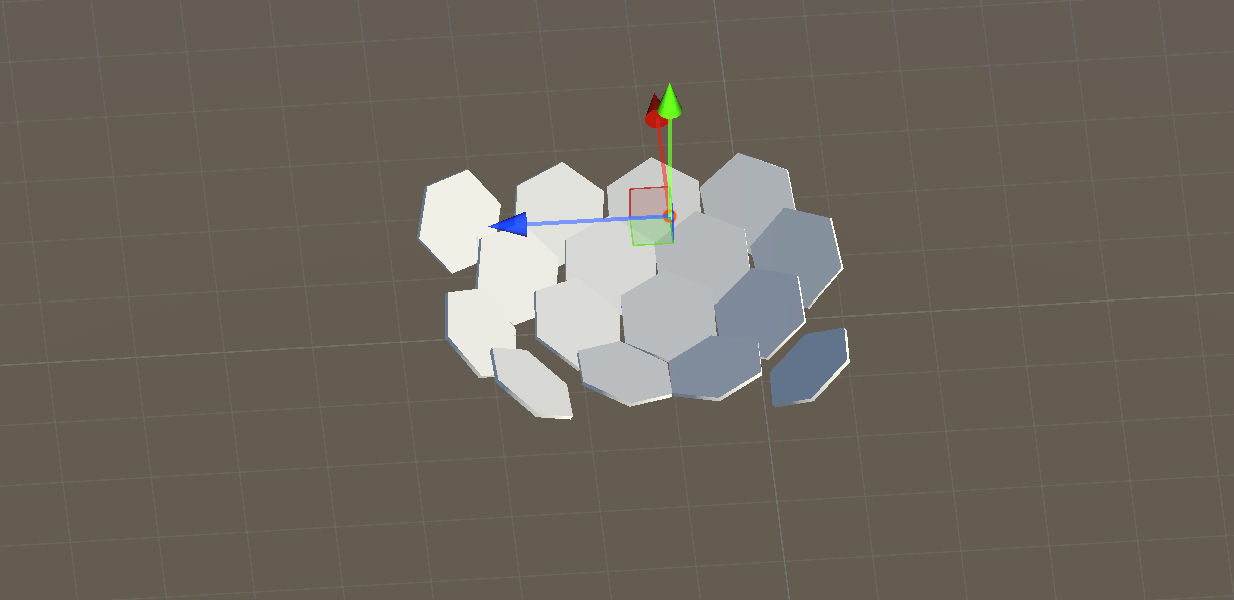
\includegraphics[
            width=0.47\linewidth,
            trim=0.25in 0 0.25in 0,
            clip
        ]{figures/fig_sim_4}
    }

    \par\vspace{2mm}

    % Row 3
    \subfloat[]{
        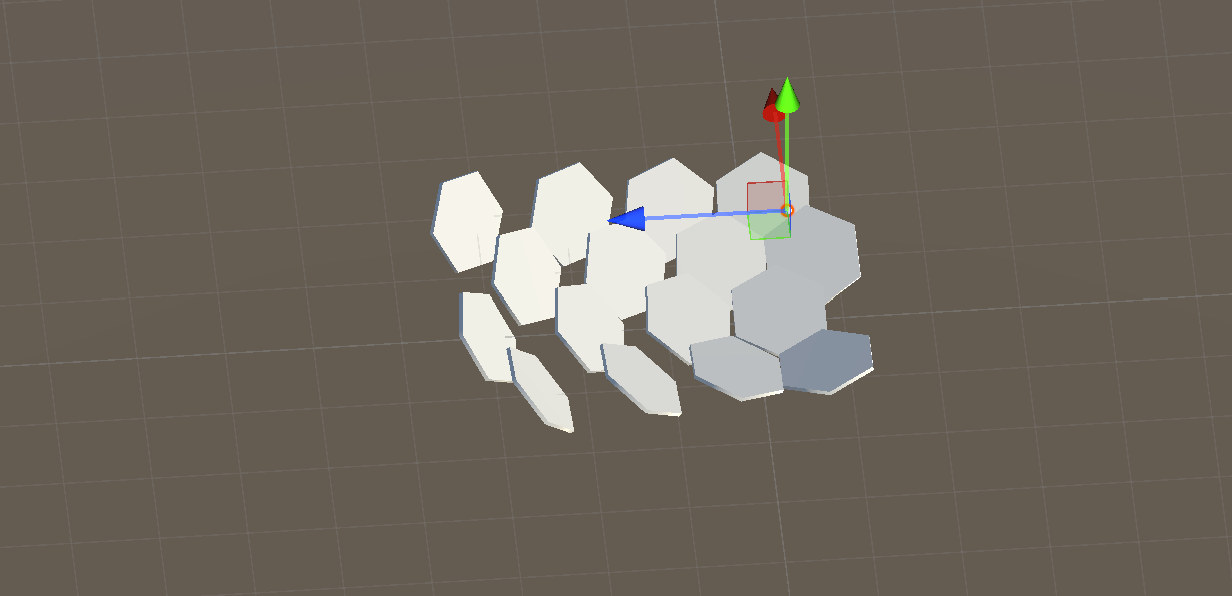
\includegraphics[
            width=0.47\linewidth
        ]{figures/fig_sim_5}
    }
    \hfill
    \subfloat[]{
        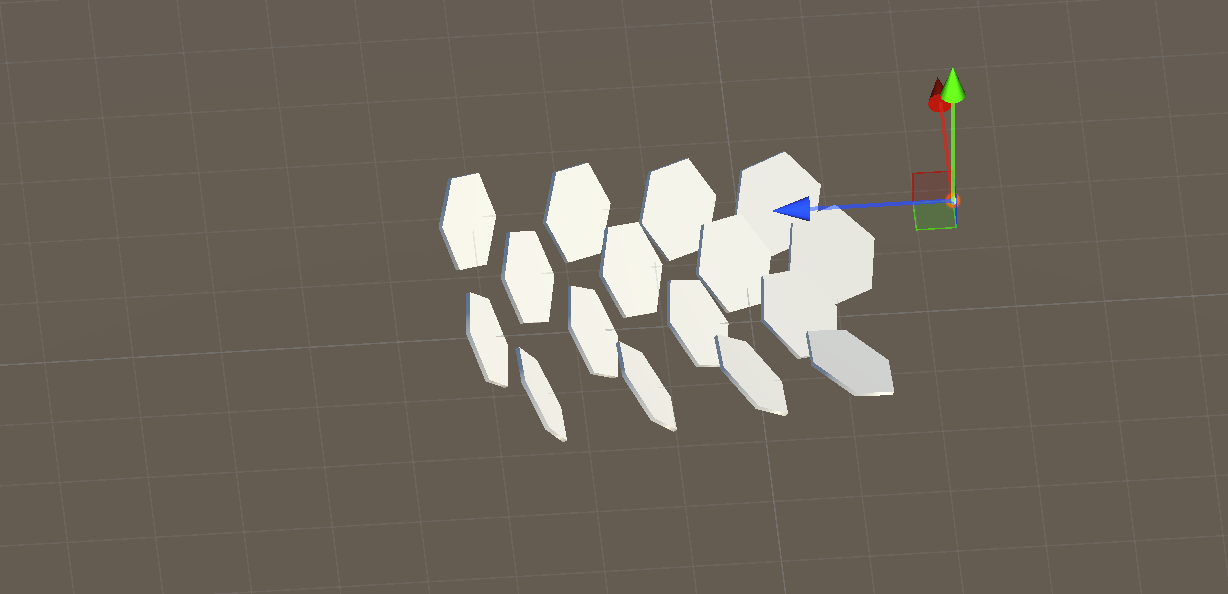
\includegraphics[
            width=0.47\linewidth
        ]{figures/fig_sim_6}
    }

    \caption{Representative frames of the SOFIA kinematic tracking
    simulation. The six frames illustrate the progressive
    reorientation of the 16-module honeycomb array as the target
    coordinate $\mathbf{p}(t)$ moves through the workspace, with the
    module normal vectors $\hat{r}_{2,3}^{(i)}$ oriented toward the
    target.}

    \label{fig:sofia_simulation}
\end{figure}

%=================================================================
\section{Discussion}
\label{sec:discussion}

The experimental characterization of the MG90S servomotor and the kinematic tracking simulation of the SOFIA kinetic array provide key insights into the intersection between high-level human-robot interaction and low-level electromechanical constraints:
\begin{itemize}
\item \textbf{Actuator Thermal Dynamics and Bang-Bang Analogy:} The empirical thermal response confirms that COTS servomotors operating under persistent position error display behavior characteristic of unconstrained saturation. Because the internal microcontroller continuously activates the H-bridge at full pulse width to overcome the perceived spatial error, electrical energy is dissipated as heat with a time constant of $\tau \approx 80.6\text{ s}$. This steep thermal gradient directly degrades the plastic gear train retainers and motor brush assemblies when temperatures exceed $65^\circ\text{C}$.
\item \textbf{Comparison with Established Literature:} In contrast to standard modular robotic architectures~\cite{seo2019modular} that treat actuators as ideal velocity/position sources, our experimental findings emphasize that thermal accumulation is a dominant failure mode in densely packed kinetic surfaces. By incorporating watchdog current and stall thresholds, SOFIA maintains continuous social interaction~\cite{fong2003social} without exceeding safe thermal boundaries.
\item \textbf{Methodological Limitations:} The LM35 sensor measures casing surface temperature rather than internal coreless rotor winding temperature directly. Internal coil temperatures are higher than outer surface measurements. Furthermore, while the external 50~Hz PWM command is known, the internal firmware closed-loop control signals remain inaccessible. Therefore, these thermal models serve as an effective macroscopic indicator rather than an internal algorithm reverse-engineering tool.
\end{itemize}

%=================================================================
\section{Conclusions}
\label{sec:conclusions}

This paper presented the conceptual design, system architecture, and experimental actuator characterization of SOFIA, an interactive modular robotic surface comprising sixteen 2-DOF electromechanical units. By coupling real-time computer vision (MediaPipe 3D upper-body pose and 21-point hand tracking) with distributed ESP32-C3 / PCA9685 motion controllers, the platform synthesizes intuitive kinetic responses to human non-verbal gestures. Experimental evaluation under persistent position error conditions demonstrated that unmitigated mechanical stalls lead to rapid thermal runaway with an identified first-order time constant of $\tau \approx 80.6\text{ s}$ and casing temperatures reaching $70.2^\circ\text{C}$. Incorporating angular limits and thermal watchdog timeouts mitigates actuator burnout risk, establishing a robust foundation for the physical implementation and deployment of modular kinetic surfaces.

%=================================================================
%% Back matter sections. IEEE does not require special macros for
%% this -- they are simple unnumbered sections before Acknowledgment.
%% Include them when your journal/course requires them; if they do
%% not apply, they can be omitted or left as "Not applicable".

\section*{Author Contributions}
P. C.-V. conceived the SOFIA platform architecture, designed the physical modular hardware, and performed the thermal characterization experiments. J. R.-G. developed the computer vision tracking pipeline, MediaPipe integration, and Unity kinematic simulation. A. M.-L. implemented the distributed ESP32-C3 firmware and RS-485 communication bus. All authors contributed to the data analysis, drafting, and critical revision of the manuscript.

\section*{Data Availability}
The experimental actuator logs, CAD models, and kinematic tracking software supporting the findings of this study are openly available in the GitHub project repository: \url{https://github.com/PaolaCV14/IOT-SOFIA-2026}.

\section*{Acknowledgment}
The authors thank the Department of Technological and Industrial Processes and the Laboratory of Distributed Systems and Telematics (LabDST) at ITESO for providing laboratory instrumentation, computing resources, and technical support throughout the development of the SOFIA project.

\section*{Conflicts of Interest}
The authors declare no conflicts of interest.

%=================================================================
\balance

\bibliographystyle{IEEEtran}
\bibliography{bibliography}

%=================================================================
%% Optional appendix -- uncomment if needed.
%\appendix
%\section{Appendix title}
%Supplementary content that is not central to the body of the
%paper, but is necessary to reproduce or dive deeper into it (e.g.,
%long mathematical derivations, raw data, code). Appendix figures and
%tables are numbered as Figure A1, Table A1, etc., and must be cited
%in the main text.

%=================================================================
%% Author biographies (optional, common in some IEEE journals).
%\begin{IEEEbiographynophoto}{First Last}
%Brief biography without a photo: education, research interests.
%\end{IEEEbiographynophoto}
%
%\begin{IEEEbiography}[{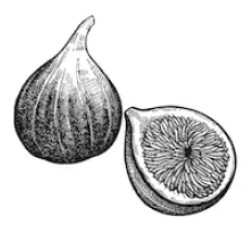
\includegraphics[width=1in,height=1.25in,clip,keepaspectratio]{fig1}}]{First Last}
%Brief biography with a photo: education, research interests.
%\end{IEEEbiography}

\end{document}
